\chapter{Experimentación y resultados}\label{chapter:experimentation}

En este capítulo se procede al cumplimiento de los objetivos principales de este trabajo. Se mostrará cómo crear y configurar un cliente en Keycloak y por último, se procede a la experimentación del sistema creado a través de un cliente realizado en \textit{Python}.

\section{Configuración de cliente Keycloak} \label{config-client}
 
%Para la ejecución de Keycloak se debe ejecutar el siguiente comando:
%
%\lstset{language=csh}
%\lstset{frame=lines}
%\lstset{caption={Ejecución de Keycloak}}
%\lstset{label={lst:runkecloak}}
%\lstset{basicstyle=\footnotesize}
%\begin{lstlisting}
%$ kc.sh start-dev
%\end{lstlisting}
%
%Por defecto \href{http://localhost:8080/}{\textcolor{blue}{http://localhost:8080/}}

Para la siguiente experimentación se ha utilizado una base de datos del Nodo Central, a la cual se accede de forma remota a través de una VPN y accediendo a una IP. La máquina en la cual se hospeda dicha base de datos tiene 1 GB de RAM y 2 CPUs lógicos virtualizados. La computadora en la que se experimentó la solución tiene 8 GB de RAM y 2.7 GHz Dual-Core Intel Core i5 de CPU.

 Luego de configurado LDAP y sincronizados los usuarios, Keycloak permite añadir clientes de forma sencilla. En las siguientes imágenes se muestra paso a paso cómo se agrega un nuevo cliente al sistema:

\begin{figure}[H]
	\centering
	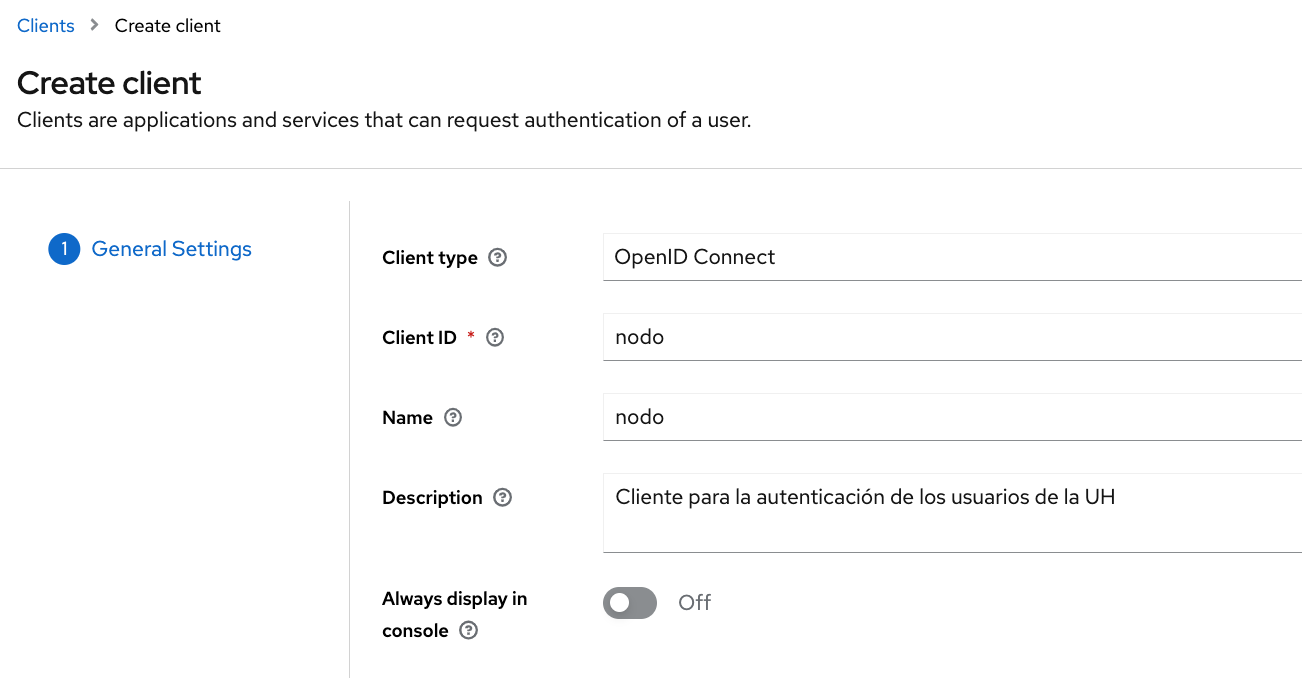
\includegraphics[width=1\linewidth]{Graphics/client_new1}
	\caption{Nuevo cliente en Keycloak(1)}
	\label{fig:clientnew1}
\end{figure}

\begin{figure}[H]
	\centering
	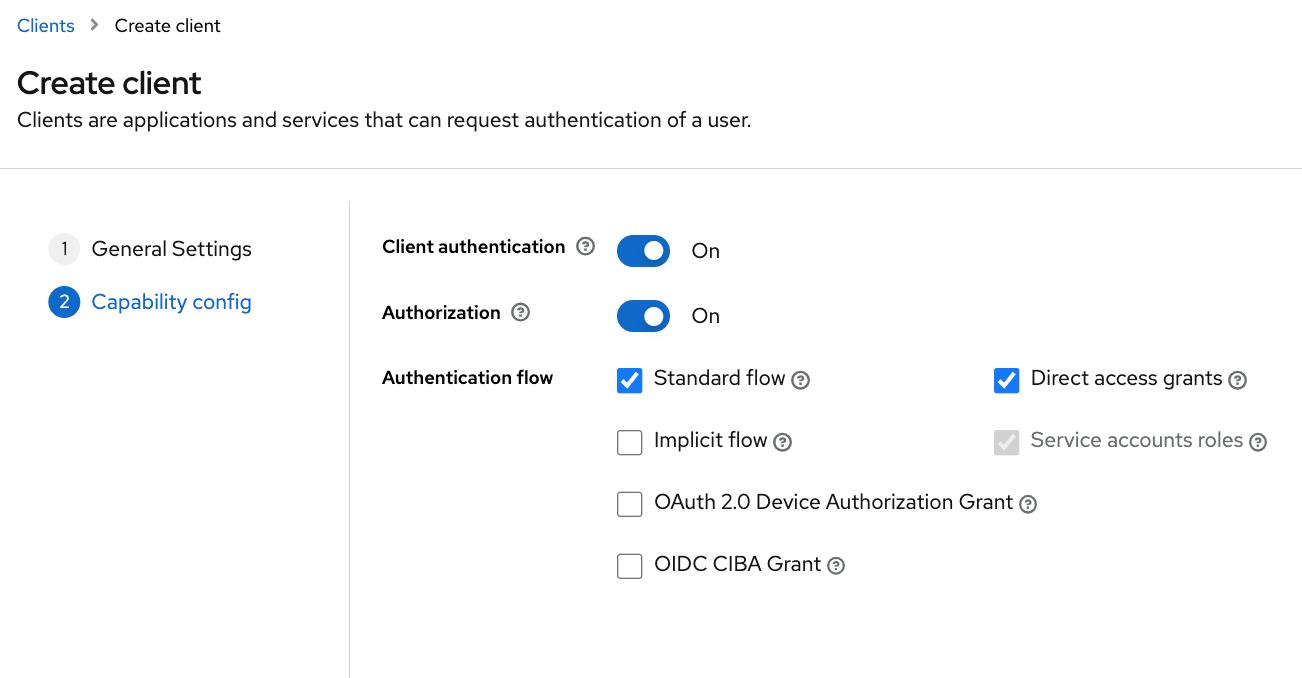
\includegraphics[width=1\linewidth]{Graphics/client_new2}
	\caption{Nuevo cliente en Keycloak (2)}
	\label{fig:clientnew2}
\end{figure}

Luego se puede ver el nuevo cliente nodo en la lista de clientes:

\begin{figure}[H]
	\centering
	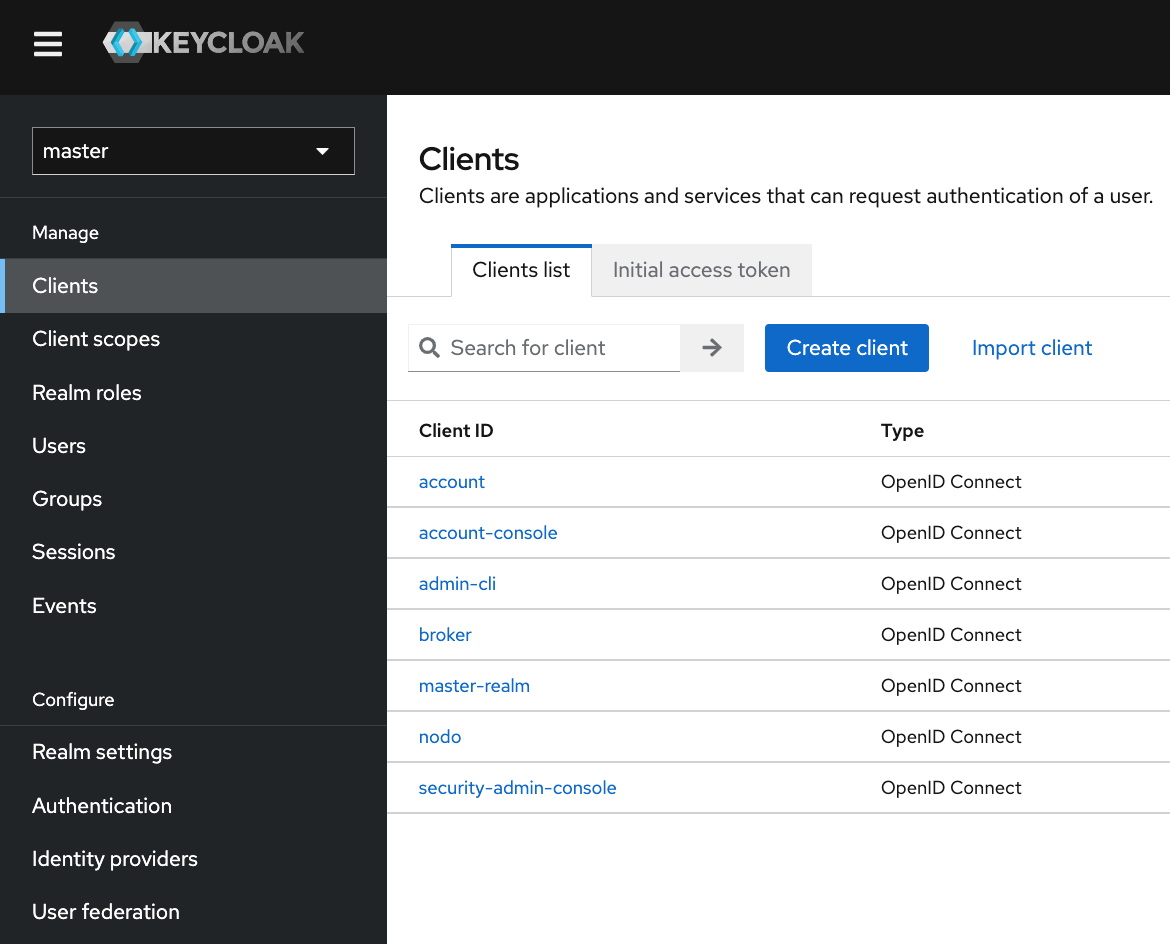
\includegraphics[width=0.9\linewidth]{Graphics/client_list}
	\caption{Lista de clientes}
	\label{fig:clientlist}
\end{figure}

Luego de crear el cliente, este se puede conectar a los servicios de Keycloak con la correcta configuración. Para ello será necesario utilizar las credenciales del cliente:

\begin{figure}[H]
	\centering
	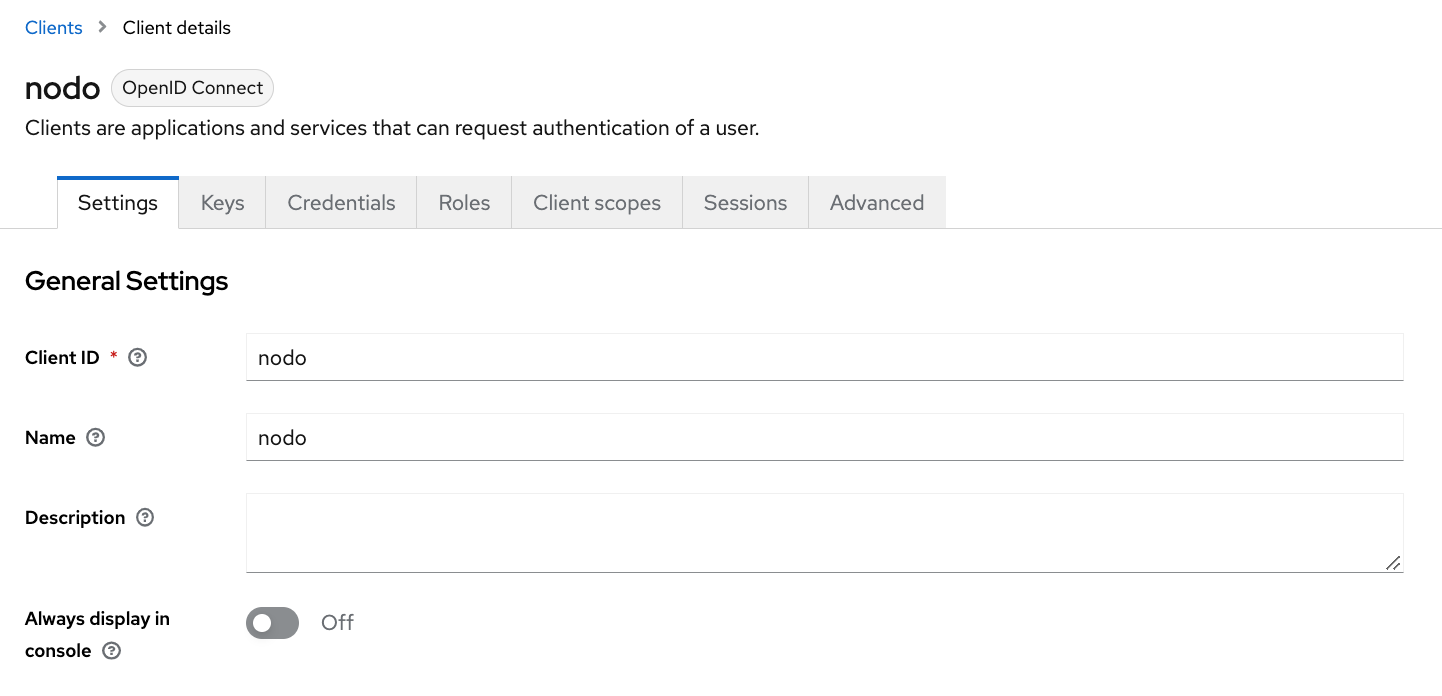
\includegraphics[width=0.9\linewidth]{Graphics/client_nodo}
	\caption{Cliente nodo}
	\label{fig:clientnodo}
\end{figure}

\begin{figure}[H]
	\centering
	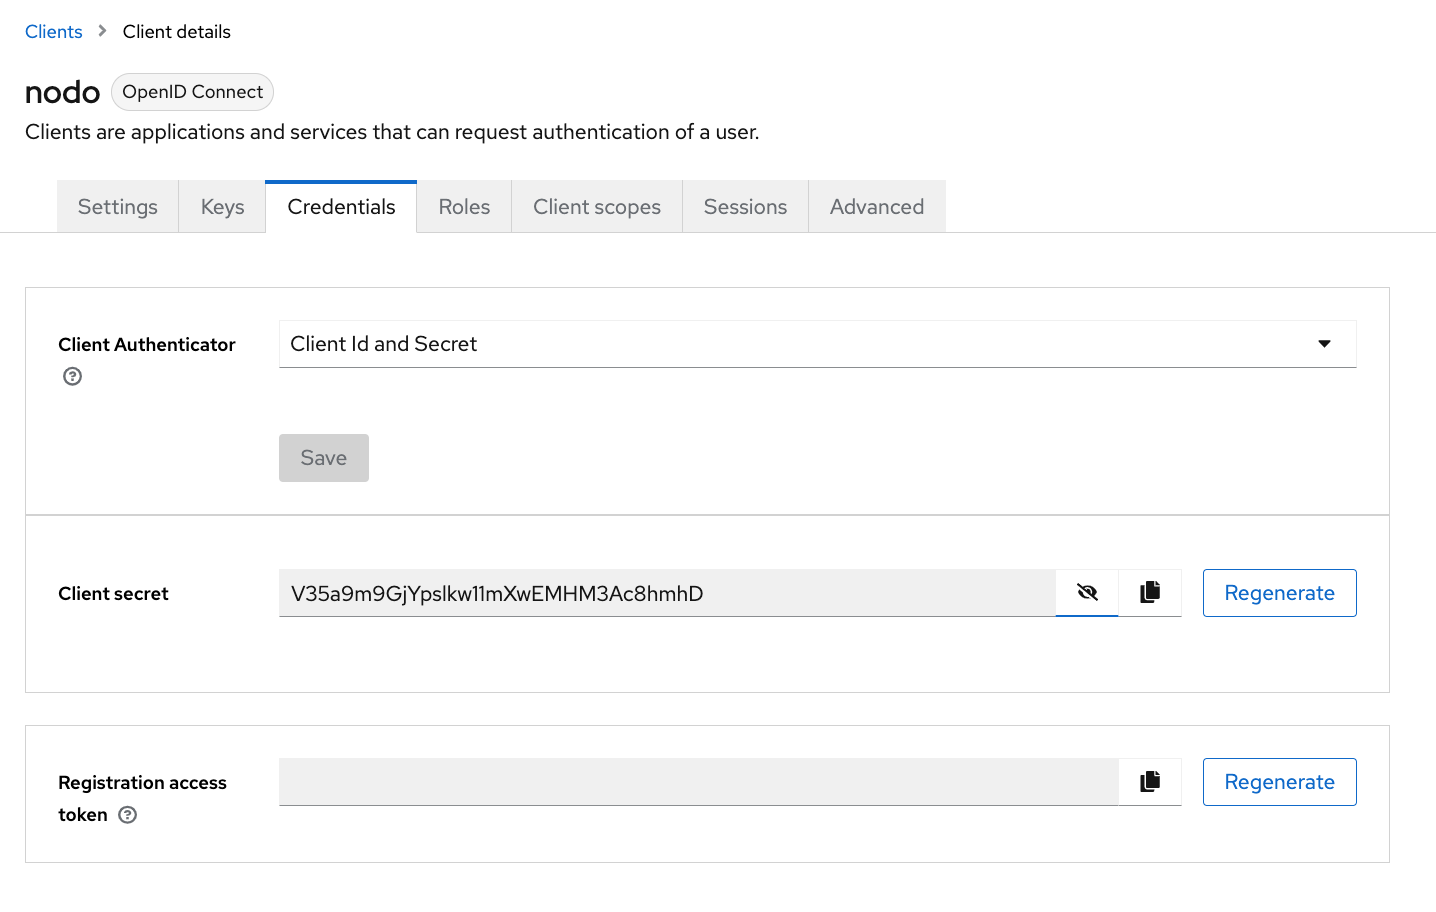
\includegraphics[width=0.9\linewidth]{Graphics/client_nodo_credentials}
	\caption{Credenciales del cliente nodo}
	\label{fig:clientnodocredentials}
\end{figure}

%\textcolor{red} {cómo se configura un cliente en keycloak?
%Qué endpoints expone la API de keycloak?
%Hablar sobre la biblioteca de python
%Poner el ejemplo de cómo se autentica}

\section{Creación de cliente Keycloak para obtención de \textit{tokens}}

En el siguiente código se muestra cómo se puede conectar el cliente a Keycloak a través de la biblioteca \textbf{python-keycloak}. También se crea una interfaz básica con Flask para visualizar los resultados.


\lstset{language=Python}
\lstset{frame=lines}
\lstset{caption={Conexión de cliente a Keycloak}}
\lstset{label={lst:code_direct}}
\lstset{basicstyle=\footnotesize}
\begin{lstlisting}
from flask import Flask
from flask import Flask, render_template, request
from keycloak.keycloak_openid import KeycloakOpenID
from keycloak.exceptions import KeycloakAuthenticationError, KeycloakGetError

import json

app = Flask(__name__)

keycloak_open_id = KeycloakOpenID(server_url="http://localhost:8080/", 
	client_id="nodo", 
	realm_name="master", 
	client_secret_key="secret key")
keycloak_open_id.well_know()

@app.route('/login', methods=['POST', 'GET'])
def login():
	error = None
	if request.method == 'POST':
		username = request.form['username']
		success, result = valid_login(username, request.form['password'])
		if success:
			return log_the_user_in(username, result["access_token"], result["refresh_token"])
		else:
			error = result["error_description"]
	# The code below is executed if the request method
	# was GET or the credentials were invalid
	return render_template('login.html', error=error)

def valid_login(username, password):
	# import pdb
	# pdb.set_trace()
	try:
		token = keycloak_open_id.token(username, password)
	except (KeycloakAuthenticationError, KeycloakGetError) as e:
		return False, json.loads(e.error_message)
	return True, token

def log_the_user_in(username, token, refresh_token):
	return render_template('success.html', username=username, token=token, refresh_token=refresh_token)
\end{lstlisting}


El código anterior genera la siguiente interfaz:

\begin{figure}[H]
	\centering
	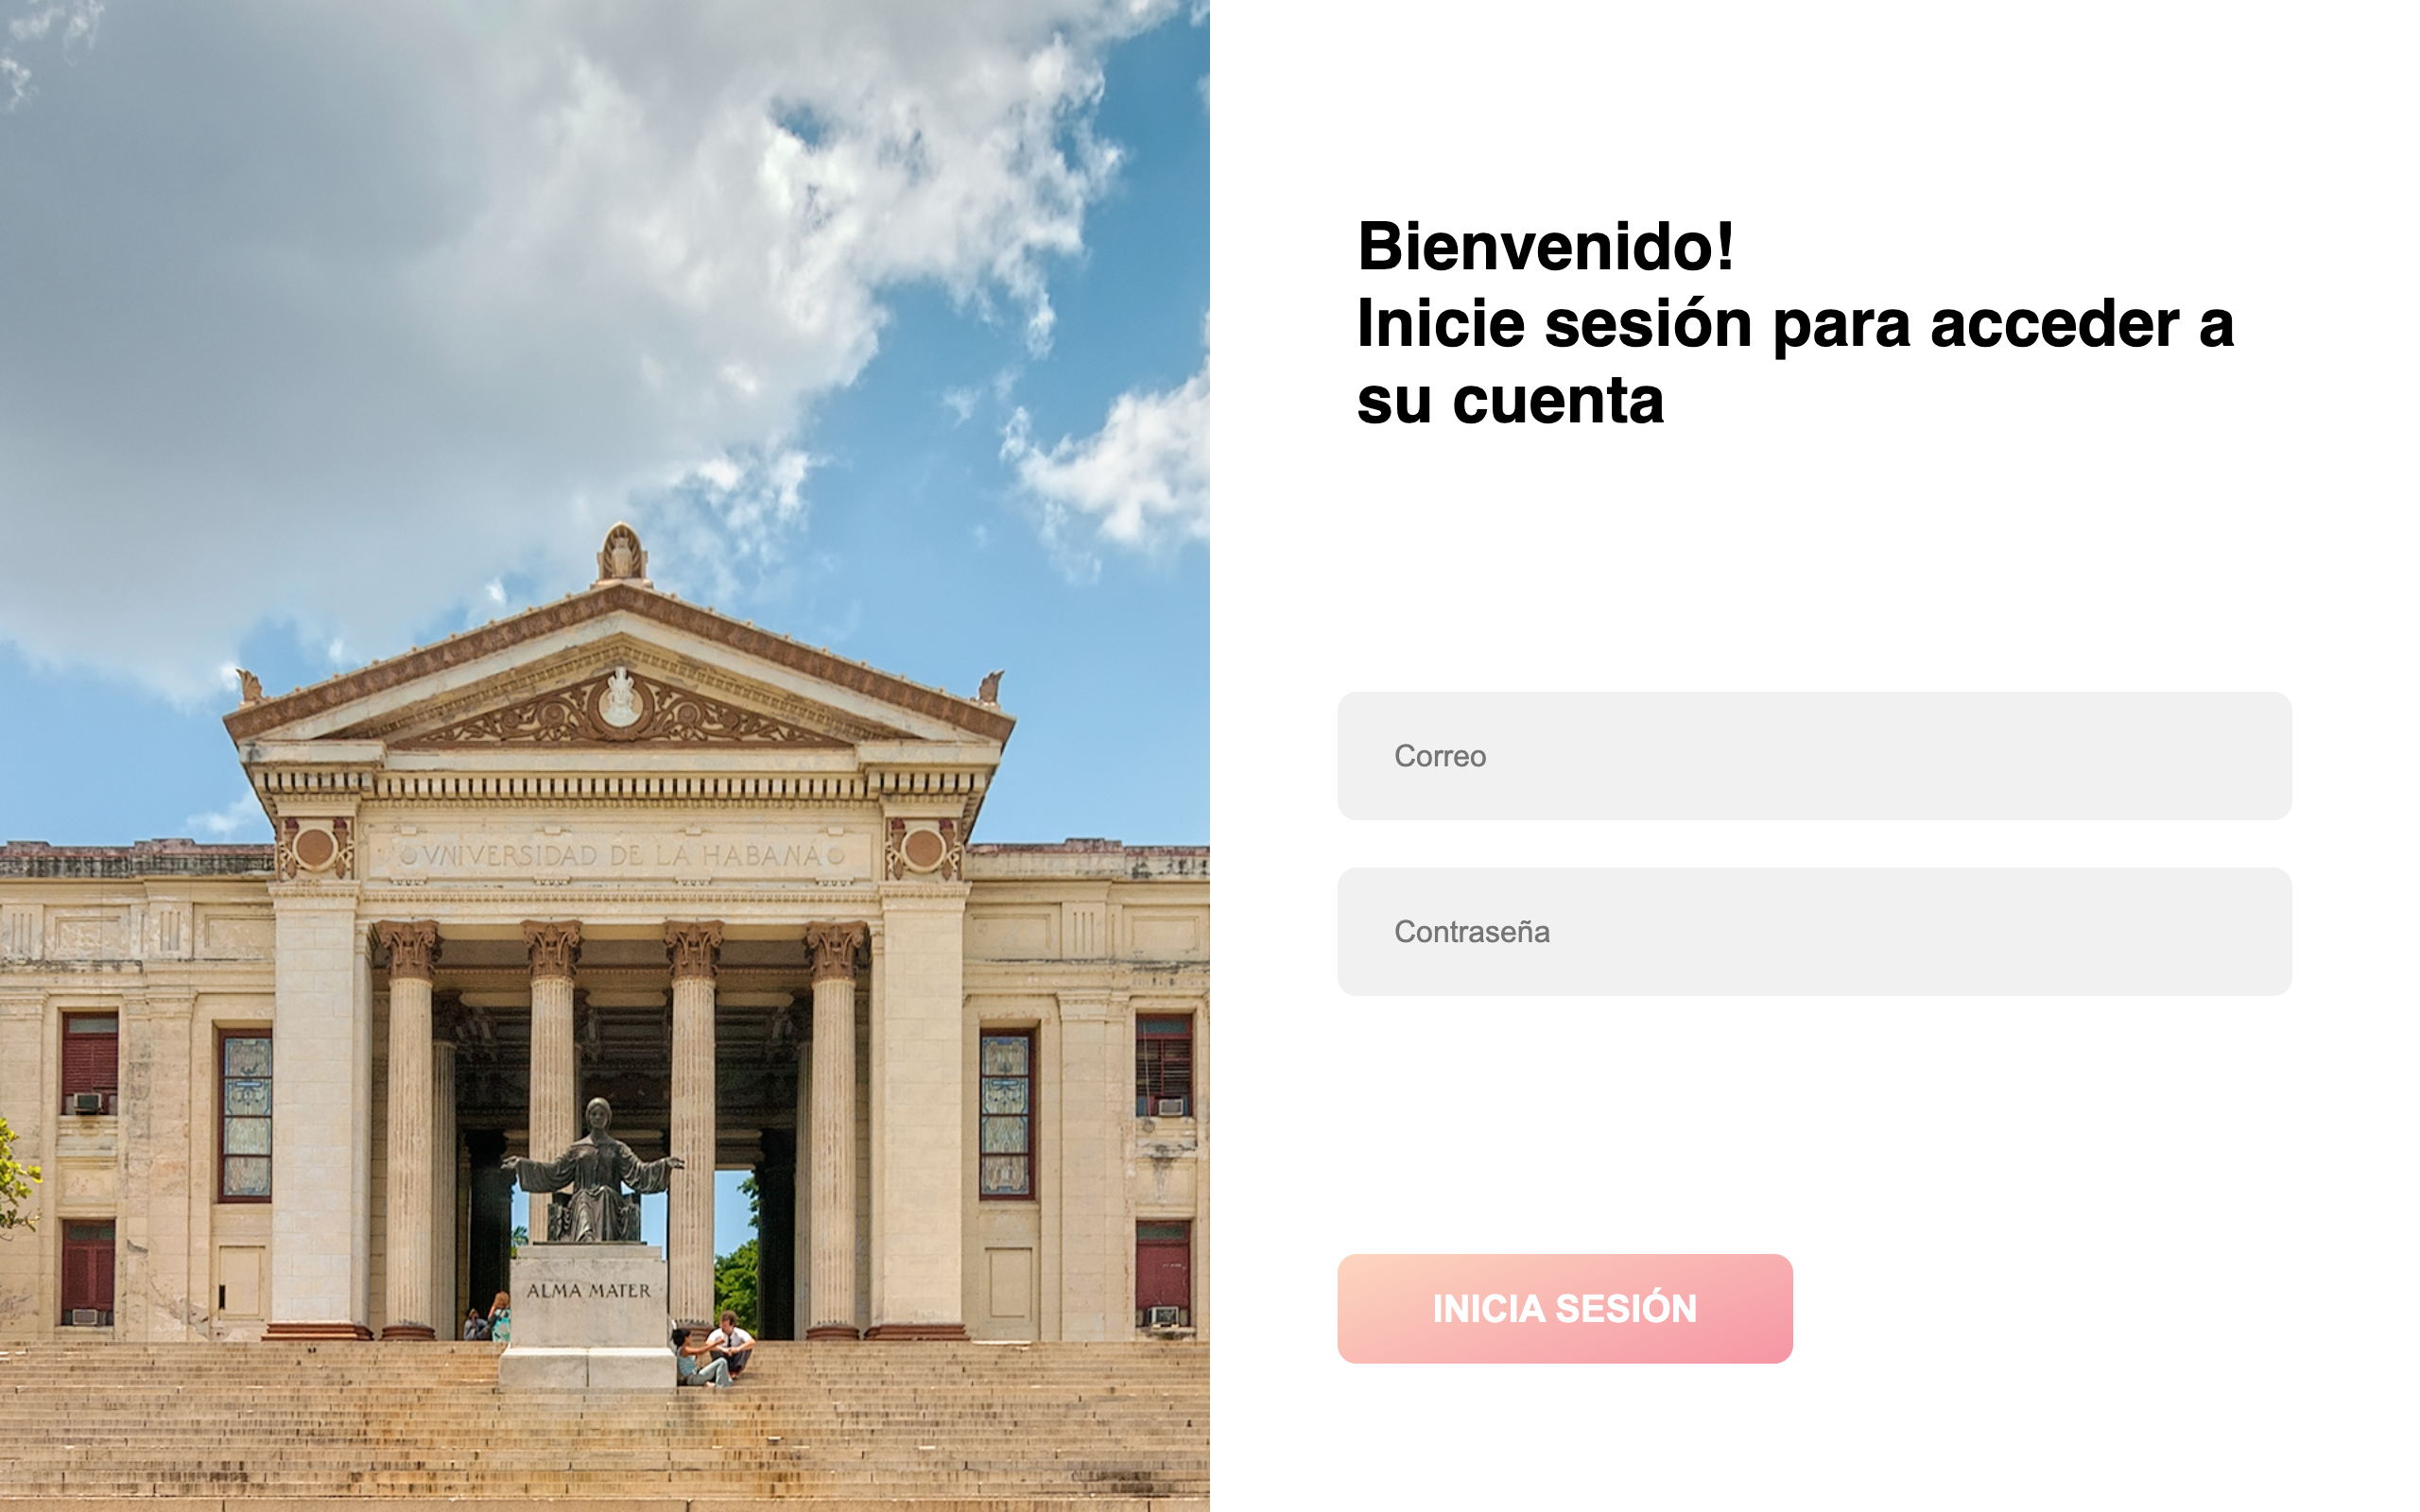
\includegraphics[width=1\linewidth]{Graphics/interfaz}
	\caption{Interfaz visual}
	\label{fig:interfaz}
\end{figure}

Luego de introducir un correo y su correspondiente contraseña se obtiene el \textit{token} de autenticación y el \textit{refresh token}:

\begin{figure}[H]
	\centering
	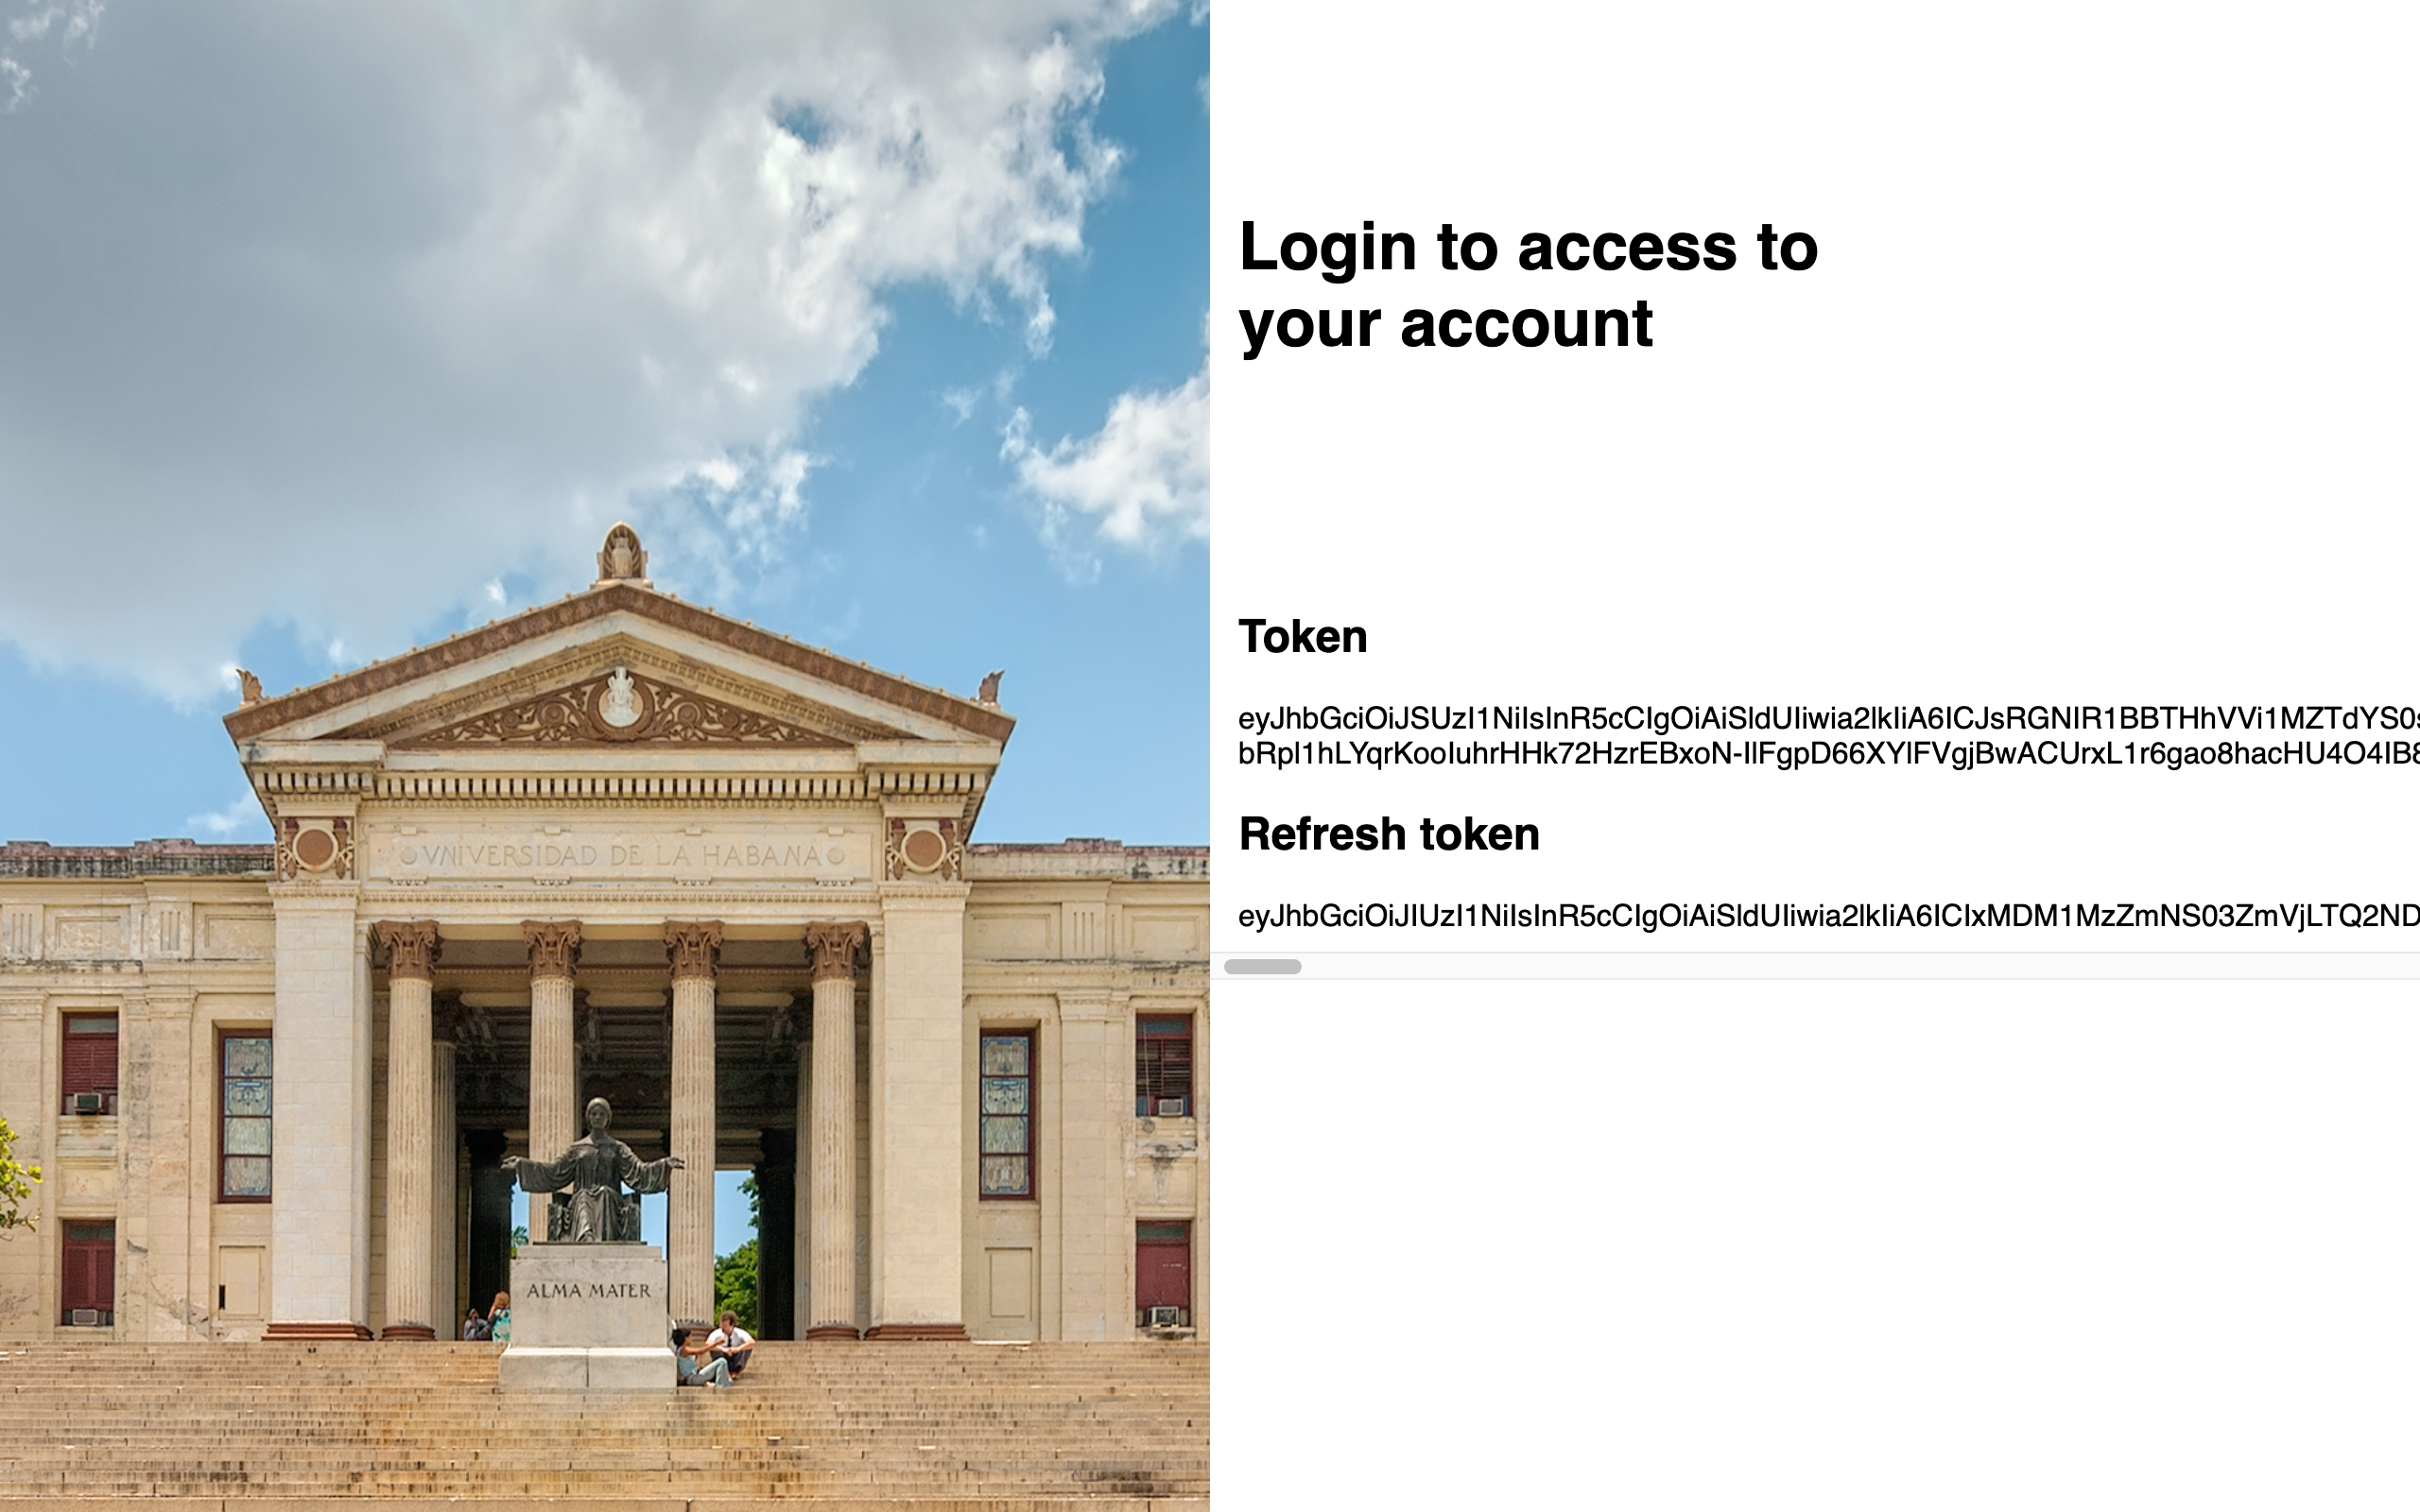
\includegraphics[width=1\linewidth]{Graphics/interfaz_token_success}
	\caption{Resultado de autenticación exitosa}
	\label{fig:interfaztokensuccess}
\end{figure}

\section{Evaluación}

Debido al alto tráfico de información al que será sometido el sistema de autenticación, se considera necesario evaluar su comportamiento. Considerando que en la universidad se cuenta con 38 678 estudiantes y 600 docentes, se asume un estimado de 50 000 usuarios en total. Para realizar las pruebas se utilizará Locust, una herramienta de código abierto para pruebas de carga. [\cite{dullmann2017caspa}] 

Locust es un software desarrollado en Python para la evaluación del comportamiento de aplicaciones web con múltiples usuarios concurrentes. Es capaz de generar tráfico que se conecta a la aplicación web con el objetivo de probar el comportamiento con una gran carga. Es una herramienta que define el comportamiento y la carga del tráfico virtual en una aplicación o en un servidor web. [\cite{pradeep2019pragmatic}]

Para evaluar el comportamiento de un sitio web con una concurrencia de 1000 usuarios, son necesarios 1000 usuarios. En la práctica es difícil disponer de 1000 personas para que abran el sitio a la vez y comprueben si este está funcionando. Locust es capaz de generar el tráfico de usuario y los resultados se representan en múltiples parámetros, incluyendo número de pedidos, tamaño de los contenidos, cantidad de intentos fallidos, entre otros.

En el siguiente código se muestra cómo conectar Locust con el sistema de autenticación creado:

\lstset{language=Python}
\lstset{frame=lines}
\lstset{caption={Conexión de Locust a Keycloak}}
\lstset{label={lst:locust}}
\lstset{basicstyle=\footnotesize}
\begin{lstlisting}
from locust import HttpUser, task
from random import choice

URL_TOKEN = "realms/{realm-name}/protocol/openid-connect/token"

class KeycloakUser(HttpUser):
def on_start(self):
self.users = [("user", "password")]
self.realm_name = "realm"
self.client_id = "client"
self.secret_key = "secret key"

@task
def token_load_test(self):
username, password = choice(self.users)
params_path = {"realm-name": self.realm_name}
payload = {
	"username": username,
	"password": password,
	"client_id": self.client_id,
	"grant_type": ["password"],
	"code": "",
	"redirect_uri": "",
	"client_secret": self.secret_key
}
self.client.post(URL_TOKEN.format(**params_path), data=payload)

\end{lstlisting}




El código anterior genera la siguiente interfaz visual:

\begin{figure}[H]
	\centering
	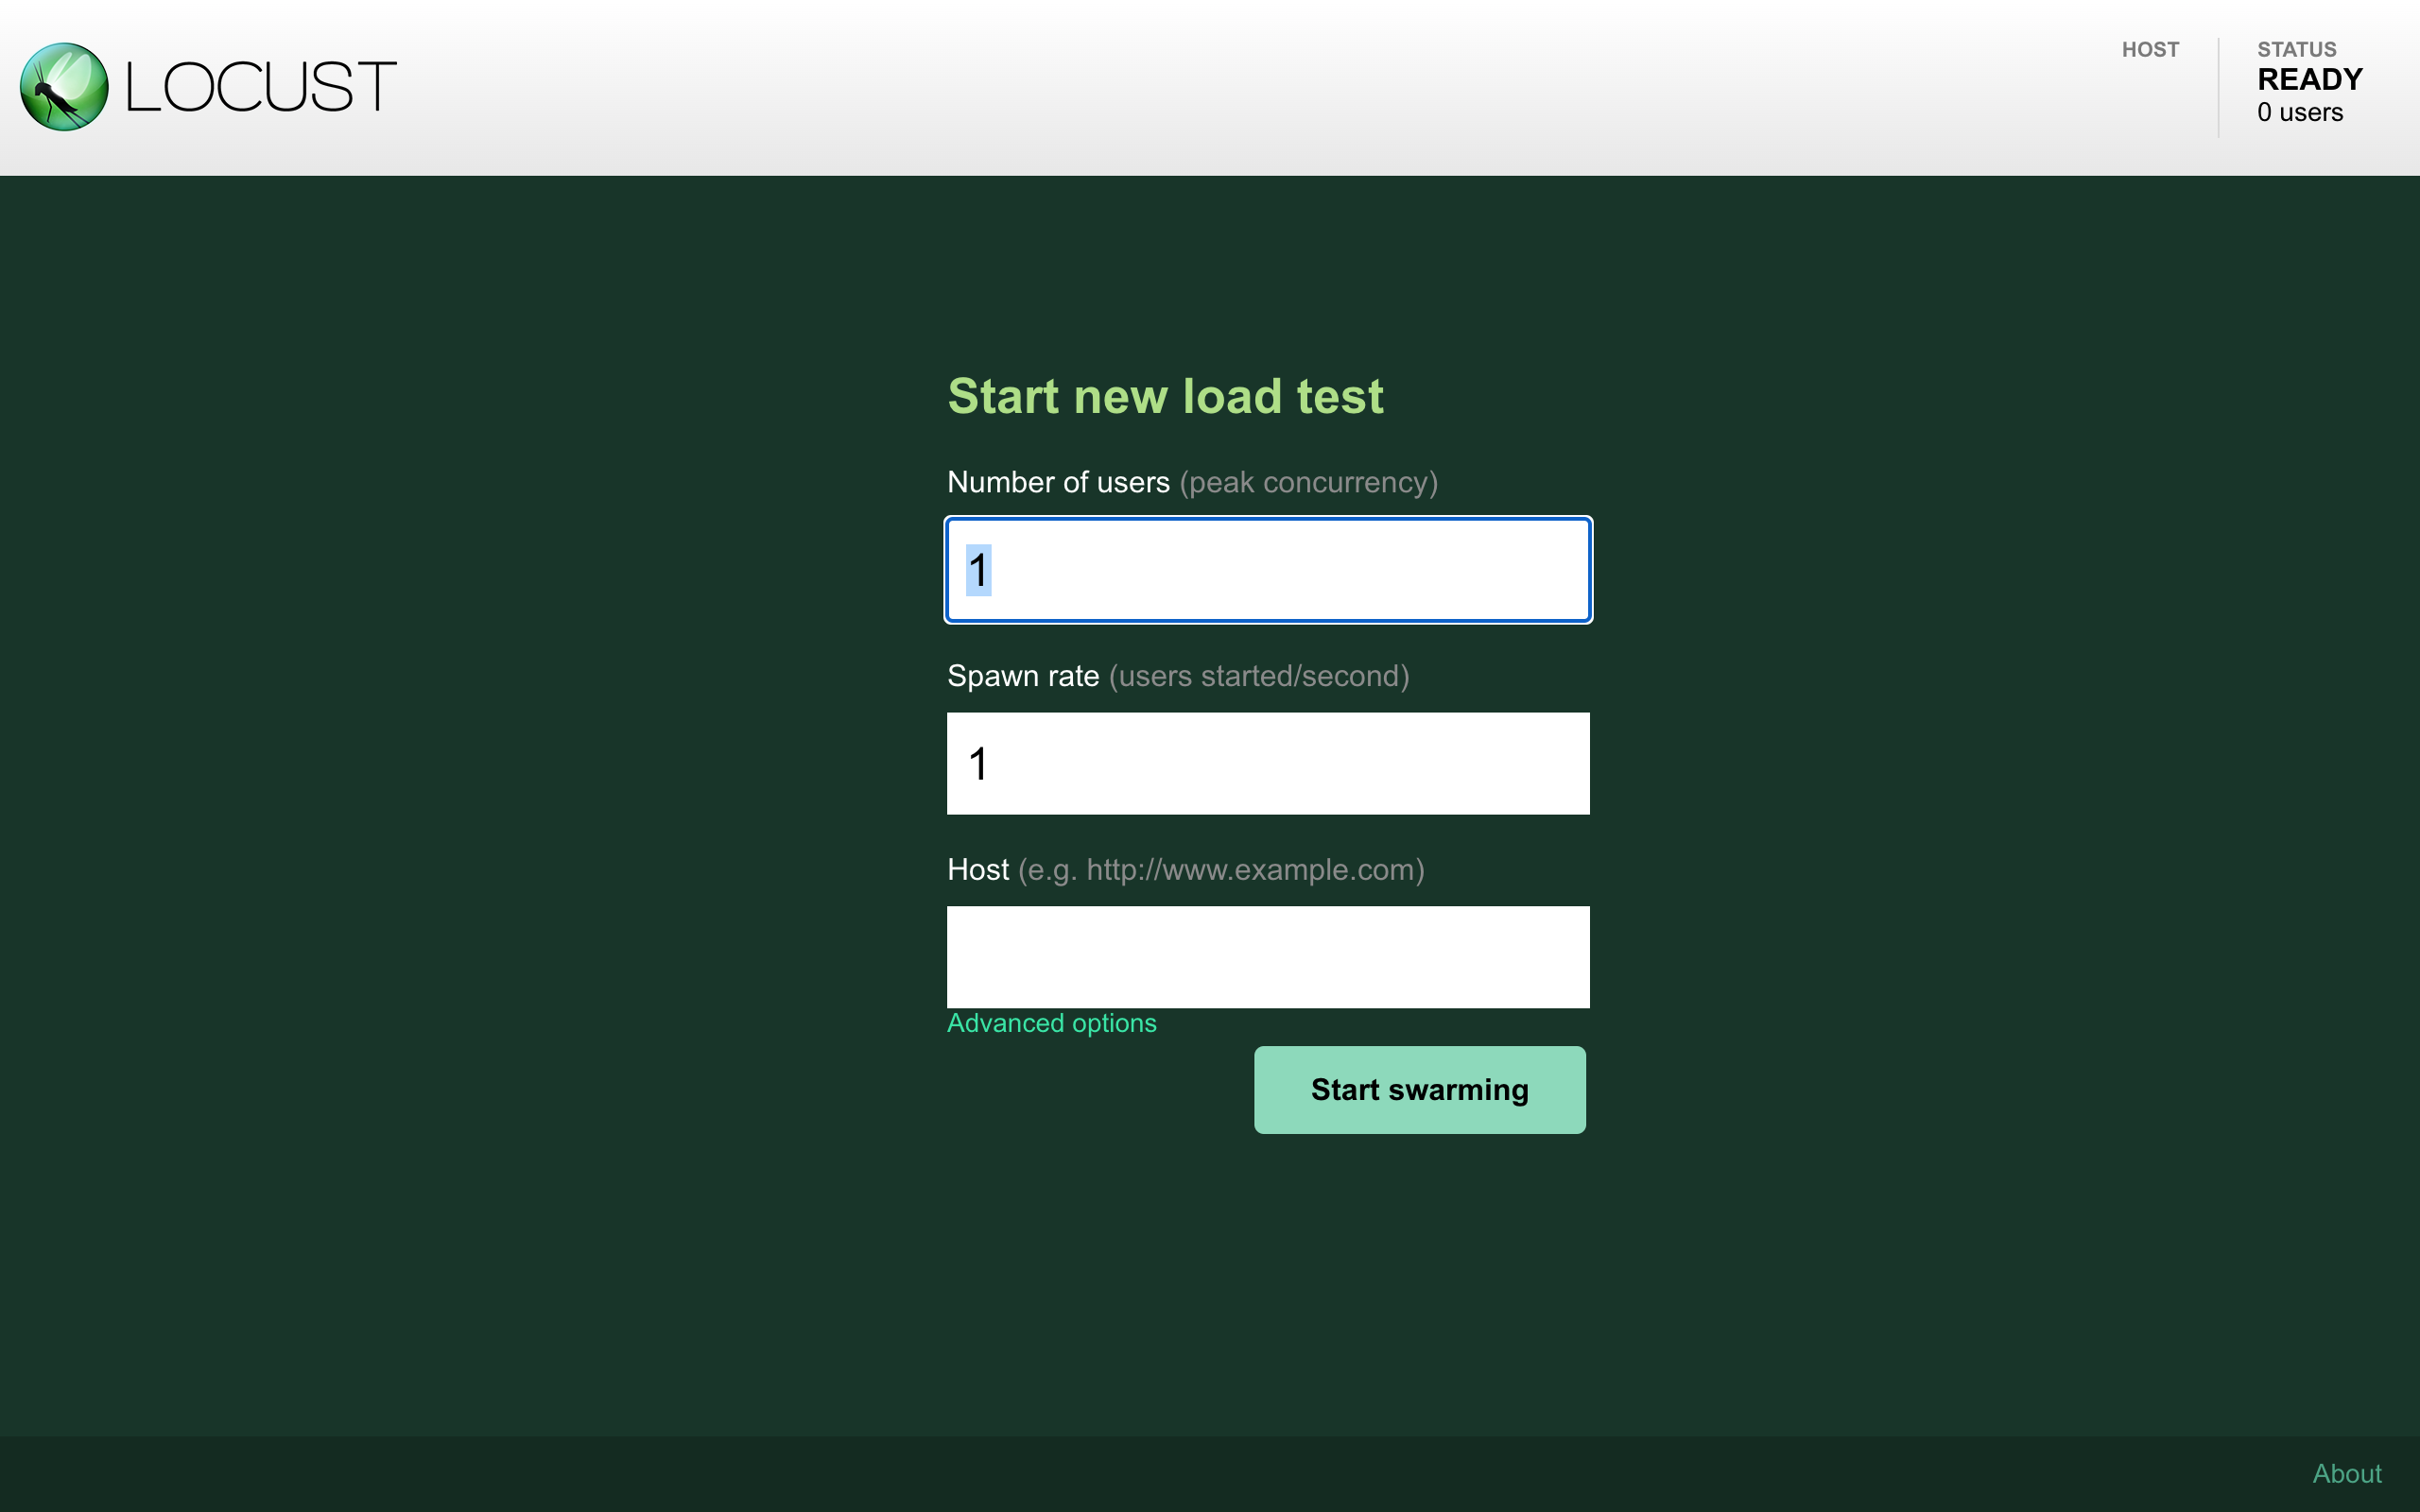
\includegraphics[width=0.9\linewidth]{Graphics/locust_visual}
	\caption{Interfaz visual de Locust}
	\label{fig:locustvisual}
\end{figure}

Con la siguiente configuración:

\begin{figure}[H]
	\centering
	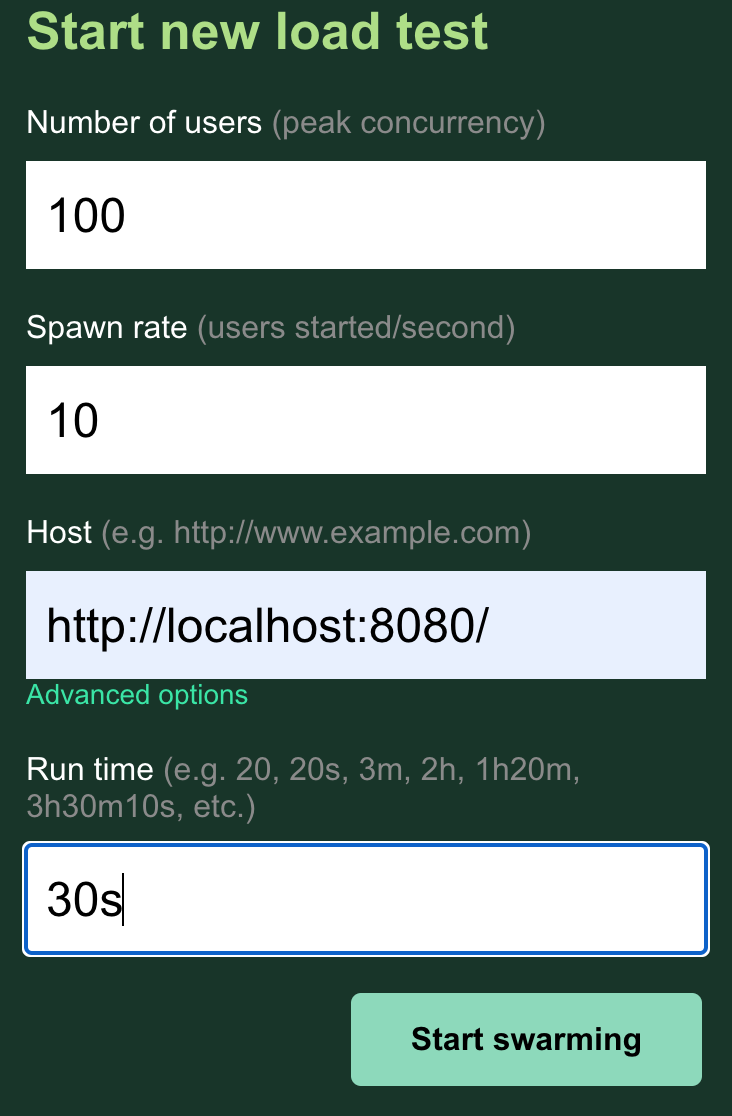
\includegraphics[width=0.3\linewidth]{Graphics/locust_config}
	\caption{Configuración de Locust}
	\label{fig:locustconfig}
\end{figure}

Se obtienen los siguientes resultados:

\begin{figure}[H]
	\centering
	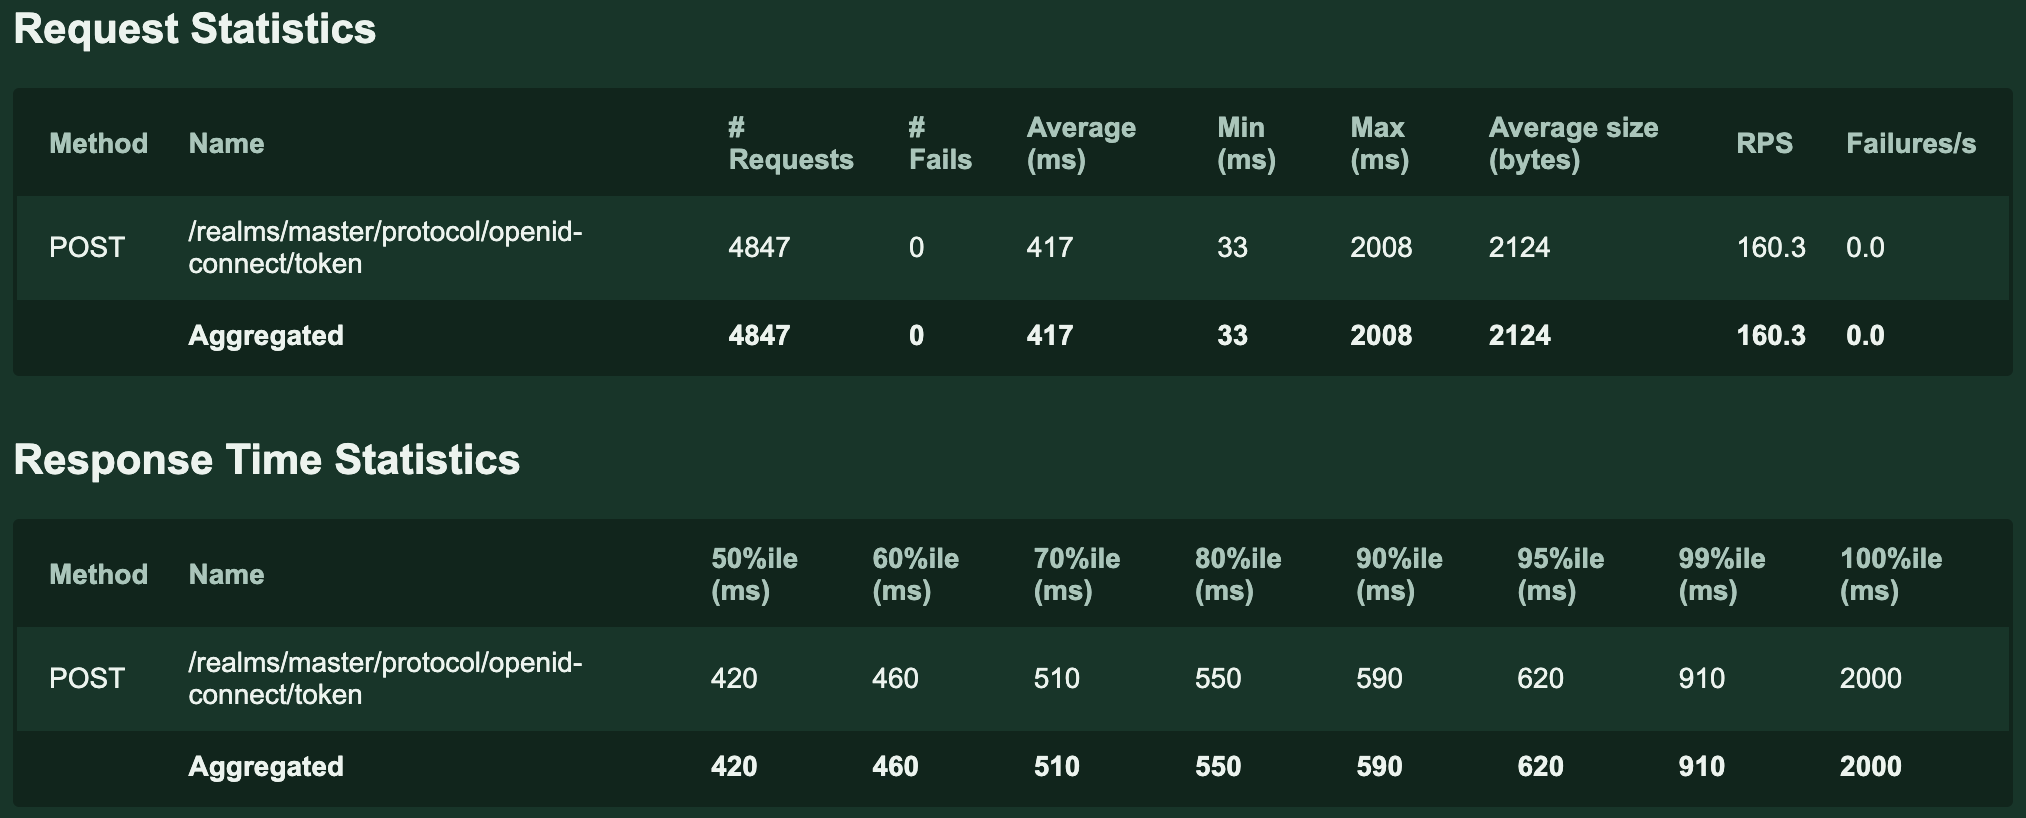
\includegraphics[width=0.9\linewidth]{Graphics/locust_statistics}
	\caption{Estadísticas obtenidas de prueba de Locust}
	\label{fig:locuststatistics}
\end{figure}

\begin{figure}[H]
	\centering
	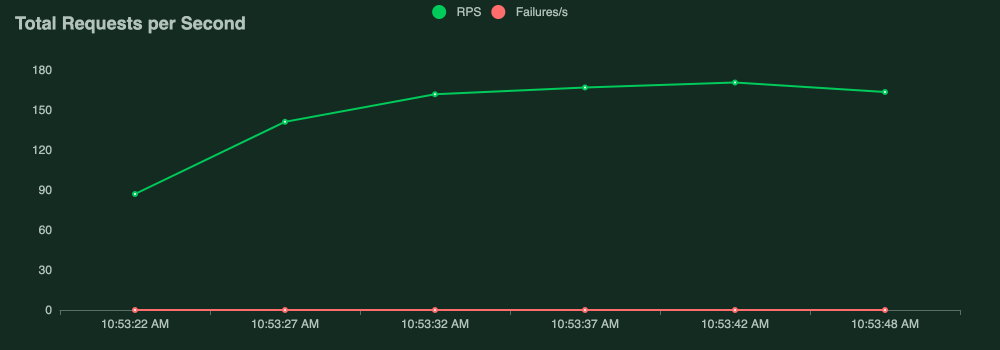
\includegraphics[width=0.9\linewidth]{Graphics/locust_total_requests_per_second}
	\caption{Total de pedidos por segundo}
	\label{fig:locusttotalrequestspersecond}
\end{figure}

En el gráfico anterior se muestra la cantidad de pedidos respondidos y fallidos por segundo. Se puede apreciar que el sistema es capaz de responder hasta 170 pedidos por segundo sin respuestas fallidas.

\begin{figure}[H]
	\centering
	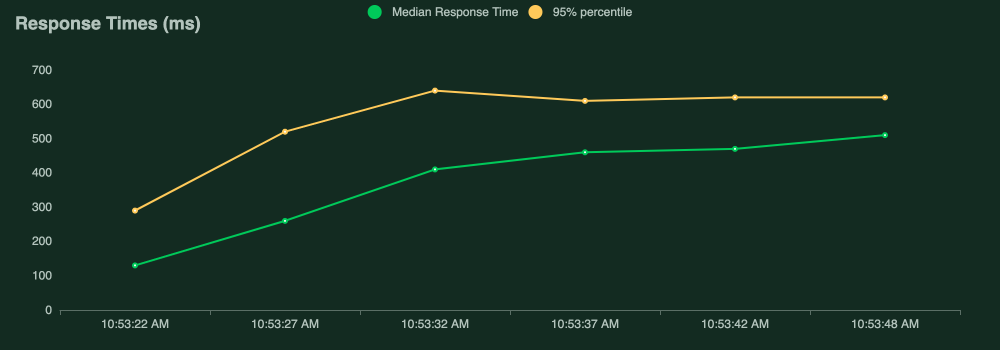
\includegraphics[width=0.9\linewidth]{Graphics/locust_response_times_(ms)}
	\caption{Tiempo de respuesta}
	\label{fig:locustresponsetimesms}
\end{figure}

El gráfico muestra la media del tiempo de respuesta de los pedidos. Se percibe que a medida que aumentan los usuarios el tiempo de respuesta aumenta, sin embargo, este se mantiene por debajo de un segundo.

\begin{figure}[H]
	\centering
	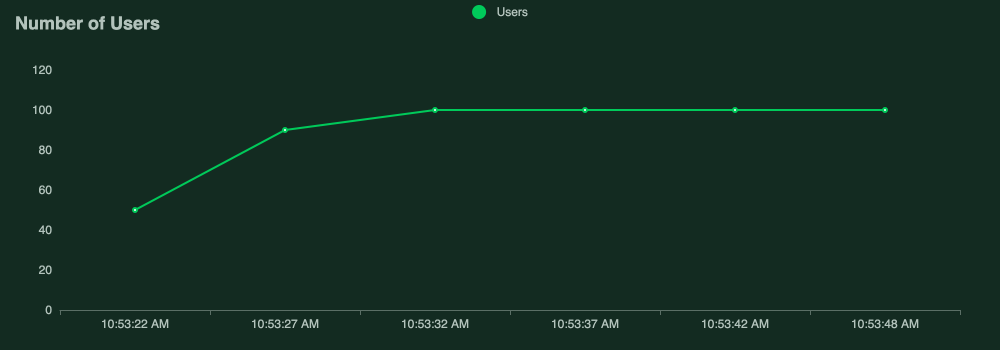
\includegraphics[width=0.9\linewidth]{Graphics/locust_number_of_users}
	\caption{Número de usuarios}
	\label{fig:locustnumberofusers}
\end{figure}

Este gráfico simula el aumento de los usuarios a lo largo del tiempo.

De la prueba de carga llevada a cabo, se puede concluir que, si el sistema es capaz de responder más de 100 pedidos por segundo, es capaz de responder al menos 360 000 pedidos por hora. Teniendo en cuenta que los \textit{tokens} de autenticación tienen una duración y en la universidad hay un estimado de 50 000 mil usuarios, se puede asumir que el sistema es capaz de interactuar con todos los usuarios de la institución accediendo a sus cuentas por 7 clientes distintos a lo largo de una hora.

 tráfico de la Universidad de La Habana.

%The Key Features of Locust includes that it is Free and Open Source under Apache with Command Line Interface (CLI) based, Evaluates both Standalone or Live Websites, Performance Testing for Web Server, Specifically for HTTP Web Server, Load Testing and Benchmarking Tool, Platform Independent and many others for the evaluation with software audit.